% +--------------------------------------------------------------------+
% | Sample Chapter 3
% +--------------------------------------------------------------------+

\cleardoublepage

% +--------------------------------------------------------------------+
% | Replace "This is Chapter 3" below with the title of your chapter.
% | LaTeX will automatically number the chapters.
% +--------------------------------------------------------------------+

\chapter{Diseño de la aplicación}
\label{makereference3}

\section{Stakeholders}
\label{makereference3.1}

\section{Escenarios}
\label{makereference3.2}

\section{Requisitos funcionales}
\label{makereference3.3}

\section{Interfaz de usuario}
\label{makereference3.4}

\section{Sistema de recomendación}
\label{makereference3.5}

\section{Prototipos}
\label{makereference3.6}

\subsection{ARCore} 
\label{makereference3.6.1} 
 
\subsection{Viro Media} 
\label{makereference3.6.2}
\begin{flushleft}
El objetivo del prototipo es reconocer imágenes almacenadas en el dispositivo para mostrar texto y
 objetos virtuales. Además de probar tecnologías de desarrollo móvil web como en este caso \textbf{React Native}
 para plataformas \textbf{iOS} y \textbf{Android}.
\end{flushleft}
\begin{flushleft}
Comenzamos construyendo una interfaz sencilla con botones que nos llevan a la escena de RA.
Para esta interfaz utilizamos \textbf{NativeBase} que es una librería que nos permite
 dar apariencia de una aplicación \textbf{iOS} y \textbf{Android} según el dispositivo.
\end{flushleft}

\begin{figure}[htb]
    \centering
    \makebox[0pt][c]{%
    \begin{minipage}[b]{0.6\linewidth}
    \centering
      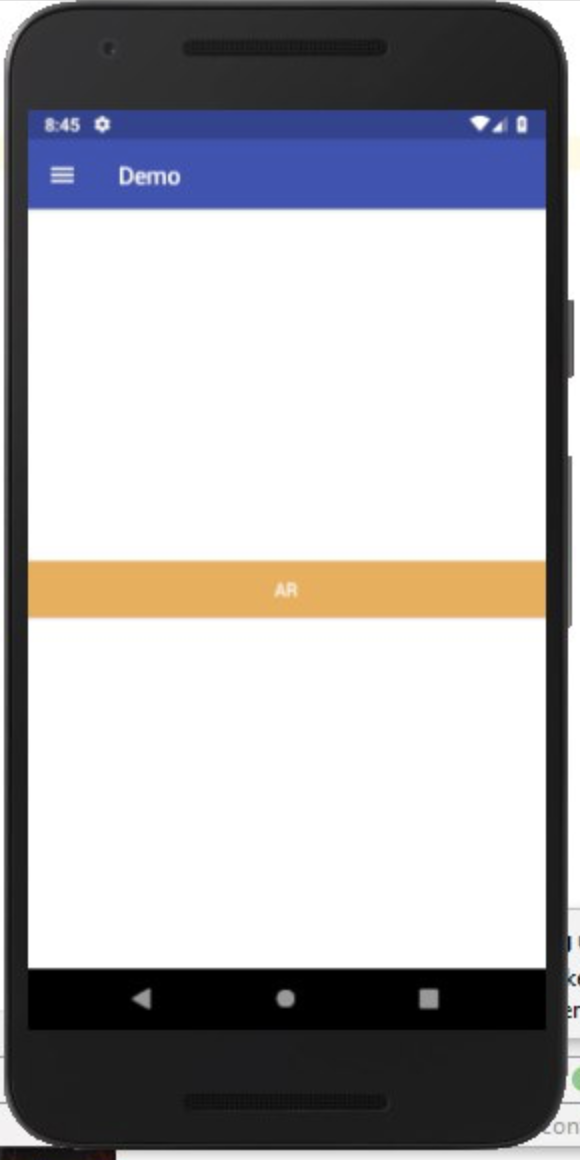
\includegraphics[scale=0.4]{figures/chapter-3/viromedia/android.png}
      \caption{Visualización con NativeBase en Android}
    \label{sva}
    \end{minipage}%
    \hspace{0.5cm}
    \begin{minipage}[b]{0.6\linewidth}
    \centering
     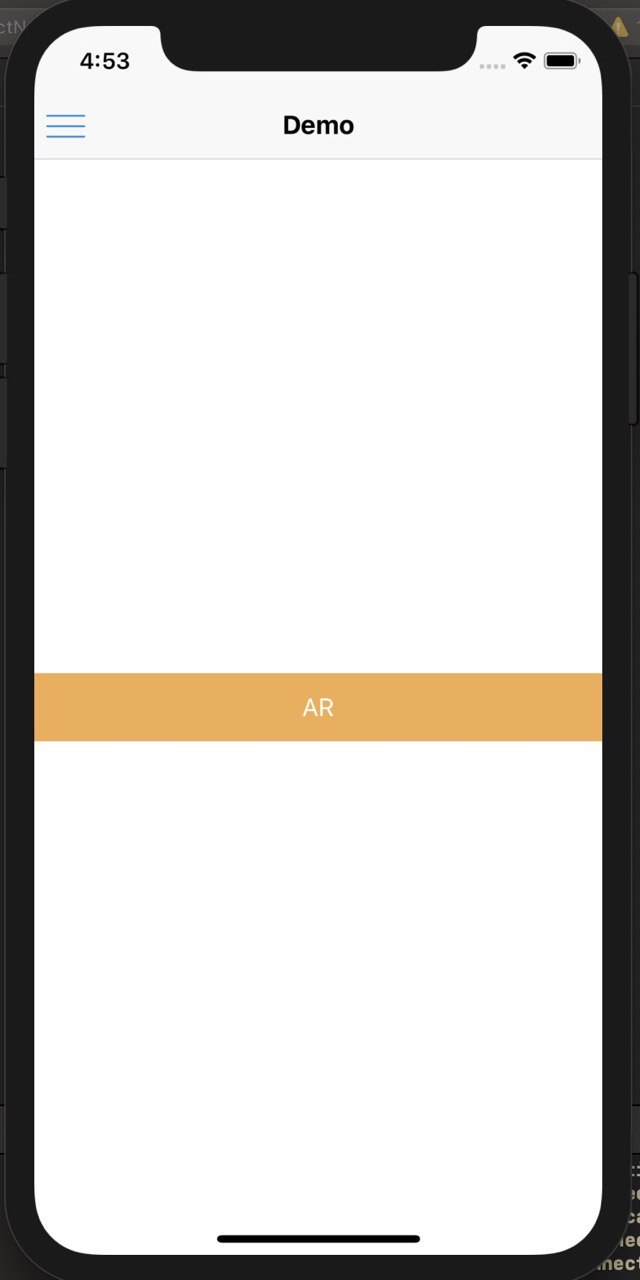
\includegraphics[scale=0.4]{figures/chapter-3/viromedia/ios.jpg}
      \caption{Visualización con NativeBase en iOS}
    \label{svb}
    \end{minipage}%
    }%
\end{figure}

\begin{flushleft}
Para la escena de realidad aumentada mostramos texto y al detectar el poster de Pantera Negra,
 reaciona mostrando una animación de dicho super heroe saliendo del póster.
\end{flushleft}
 
\begin{figure}[H]
    \centering
    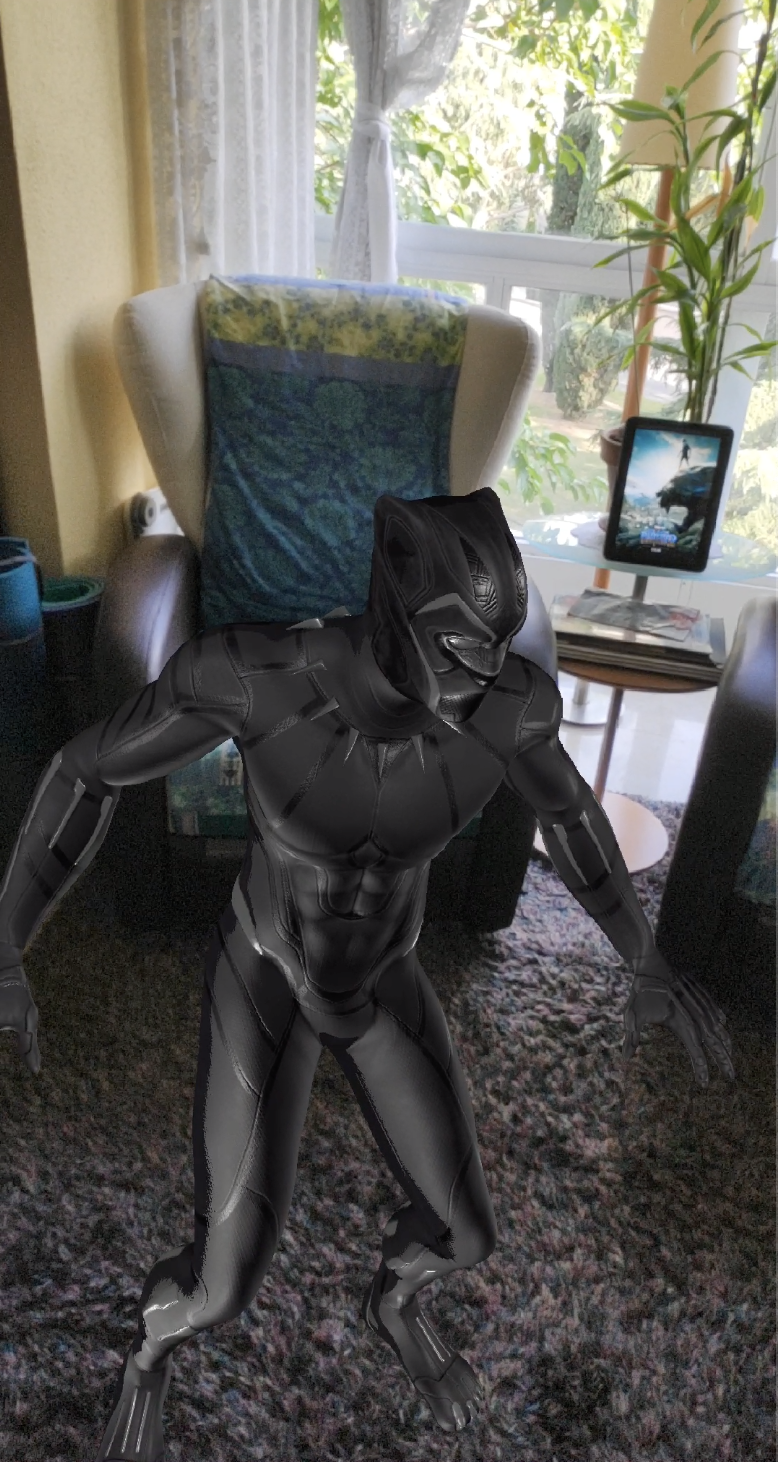
\includegraphics[width=3in]{figures/chapter-3/viromedia/blackpanther.png}
    \caption{Visualización de RA}
\end{figure}

\begin{flushleft}
Una de las ventajas que apreciamos fue la facilidad del lenguaje en este caso \textbf{Javascript}
 utilizando la popular librería \textbf{ReactJS} y la buena documentación de \textbf{Viro Media}
 que hacian que el proceso de codificación fuera agradable.
\end{flushleft}
\begin{flushleft}
Uno de los problemas es que las dependencias de \textbf{Viro Media} entran en conflicto con las de \textbf{NativeBase}
 no habiendo forma de encontrar versiones compatibles. Utilizamos las últimas que a pesar de lanzar
 advertencias funcionaba el ejemplo realizado.
Otro problema es la compilación de la aplicación, \textbf{Viro Media} tiene una aplicación para probar la
 que nosotros desarrollamos conectándose a nuestro ordenador a traves de la red. El problema es
 que algunos recursos como los iconos que utilizaba \textbf{NativeBase} no eran descargados, por lo que la
 mejor forma era probar la versión compilada de \textbf{iOS} y \textbf{Android}. La forma de compilar
 la aplicación era un proceso costoso para los ordenadores, lento y con multitud de problemas según
 se ampliaba las librerías que se utilizan.
\end{flushleft}

\begin{flushleft}
La conlusión fue que \textbf{Viro Media} y \textbf{React Native} son tecnologías muy prometedoras pero debido a los
 problemas surgidos y a que todas sus versiones no eran estables vimos un claro riesgo para
 nuestro proyecto.
\end{flushleft}

\newpage
\subsection{Vuforia + Android} 
\label{makereference3.6.3} 
 
\begin{flushleft}
En este prototipo utilizamos la librería nativa de \textbf{Vuforia} para \textbf{Android} para 
realizar las pruebas de tecnología de reconocimiento de imágenes tanto en  
local como usando la nube que nos ofrecía \textbf{Vuforia}, para la posterior renderización
de objetos y textos.

Las características tecnológicas de este prototipo son las siguientes:
\end{flushleft}

\begin{enumerate}
    \item La librería de \textbf{Vuforia} para \textbf{Android} está diseñada a muy bajo nivel.
    \item \textbf{Vuforia} para dibujar en 3D usa la librería \textbf{OpenGL}.
    \item \textbf{OpenGL} utiliza una serie de espacios donde se van colocando los elementos: 
    \begin{enumerate}
        \item \textbf{Local space}: Es el espacio local de cada objeto.
        \item \textbf{World space}: Es el mundo donde se encuentran los objetos.
        \item \textbf{View space}: El mundo visto desde la perspectiva de la cámara.
        \item \textbf{Clip space}: Se integra con la pantalla del móvil y, definiendo los límites visibles, se establecen unas coordenadas de rango (-1,-1) - (1,1).
    \end{enumerate}
    \begin{flushleft}
        Las transformaciones de estos espacios se realizan mediante matrices 4x4, 
        en las que la primera fila hace referencia a la coordenada x, la segunda a la coordenada y y la 
        tercera a la coordenada z, mientras que la última columna hace referencia a los desplazamientos 
        de los objetos en esos 3 ejes.
        \end{flushleft}
        

        
            \begin{figure}[H]
                \centering
                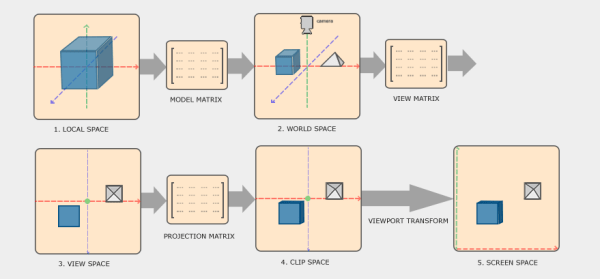
\includegraphics[width=5in]{figures/space-transformation.png}
                \caption{Esquema de los distintos espacios que usa OpenGL}
            \end{figure}

            \begin{figure}[H]
                \centering
                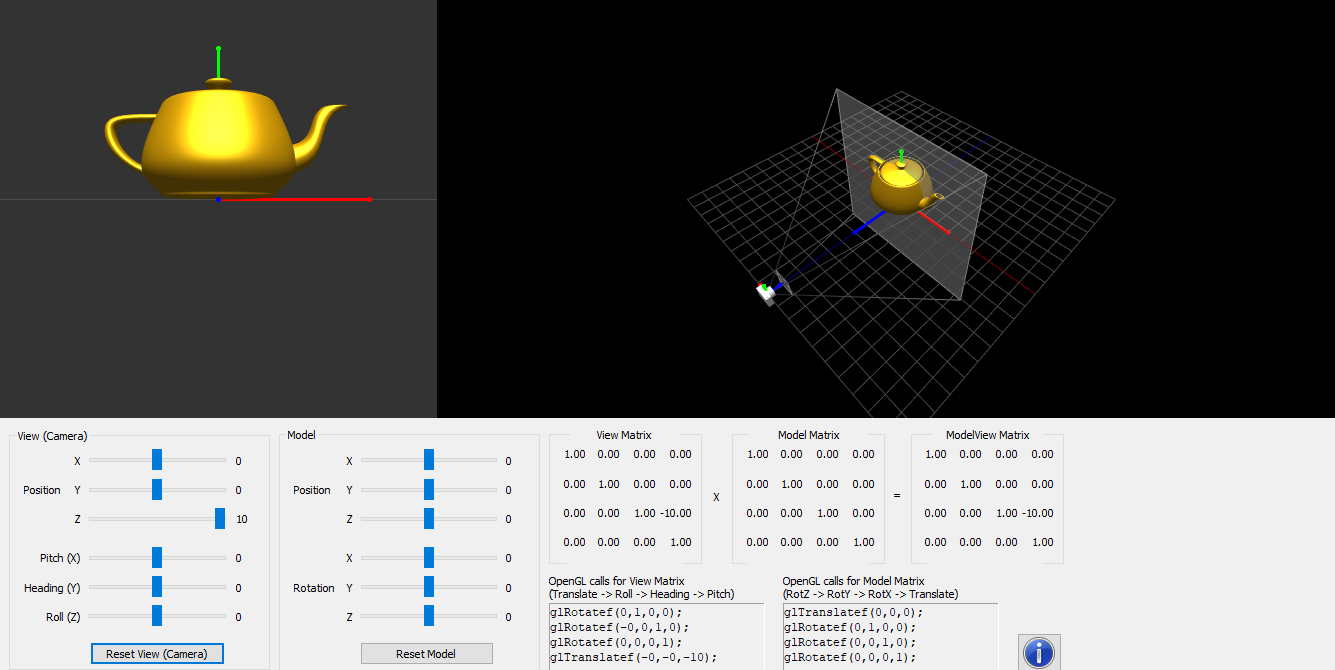
\includegraphics[width=5in]{figures/teapot.png}
                \caption{Ejemplo de un modelo en 3D}
            \end{figure}
    
    \item En \textbf{OpenGL} es necesario escribir código para que las tarjetas gráficas rendericen el modelo 3D,
    el lenguaje que se usa es \textbf{GLSL}. Este código de \textbf{GLSL} se escribe en forma de \textbf{String} y se llama a un método 
    que proporciona \textbf{OpenGL}.
    \begin{figure}[H]
        \centering
        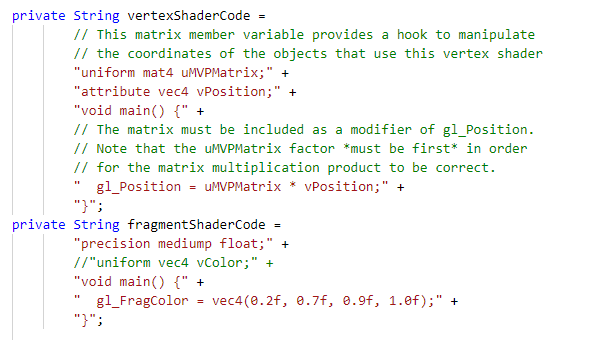
\includegraphics[width=5in]{figures/GLSL.png}
        \caption{Código en GLSL}
    \end{figure}
        
    \item Otro aspecto a tener en cuenta es que \textbf{OpenGL} solo nos ofrece lo básico, no nos ofrece métodos para dibujar 
    directamente objetos sino que hay que seguir un pipeline de procesos para conseguir dibujar algo.
    \newline
    \begin{flushleft}
    Esto consiste en pasar un \textbf{array} de números (cada tres para definir un punto) 
    a las tarjetas gráficas, establecer triángulos entre los puntos (más arrays de números) 
    definir colores a partir de los puntos (más arrays)..., y con el código del shader, ejecutar 
    estos datos.
    \begin{figure}
        \centering
        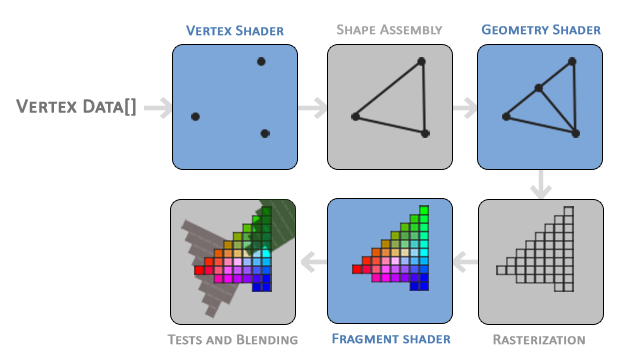
\includegraphics[width=4in]{figures/pipeline.png}
        \caption{Pipeline de la construcción de un modelo}
    \end{figure}
    \end{flushleft}
    \newpage
    \item Por último como sólo ofrece métodos básicos, no hay métodos de escritura de texto, y la forma que 
    encontramos y que funcione fue usar un bitmap con los caracteres. Rechazamos esto por un principal motivo, para hacer que funciones hay que codificar a muy bajo nivel y 
    nos costaría mucho tiempo y esfuerzo.
    \begin{figure}
        \centering
        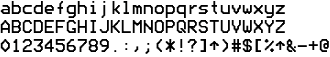
\includegraphics[width=5in]{figures/bitmap-font.png}
        \caption{Mapa de bits de caracteres usado}
    \end{figure}
\end{enumerate}
 

\newpage
\subsection{Vuforia + Unity} 
\label{makereference3.6.4}
\begin{flushleft}
    Para realizar este prototipo utilizamos Unity como herramienta básica para realizar la aplicación y Vuforia para dar soporte a la Realidad Aumentada.
    El prototipo a desarrollar consistío en un modelo 3D de un dragón que aparecía al detectar una imagen que previamente habíamos establecido como "imagen objetivo".
\end{flushleft}
    \begin{figure}[H]
        \centering
        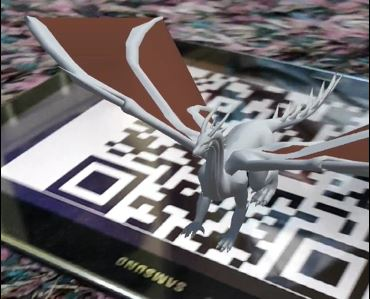
\includegraphics[width=5in]{figures/prototipoUnity.jpg}
        \caption{Modelo en 3D que aparecía al detectar la imagen}
    \end{figure}
\begin{flushleft}
    Pese a que nadie del equipo había utilizado Unity previamente el resultado fue bastante positivo ya que:
    \begin{enumerate}
    \item Unity resultó ser intuitivo y relativamente fácil de aprender las funcionalidades básicas.
    \item Vuforia parecía estar muy probada e incluía de serie muchas funcionalidades.
    \item Vuforia tenía la opción de utilizar un Cloud para almacenar las imágenes objetivo.
    \end{enumerate}
\end{flushleft}

\newpage
\subsection{Server en Spring} 
\label{makereference3.6.5}

\begin{flushleft}
    Para la realización de la parte backend de la aplicación decidimos
    incorporar la tecnología de \textbf{Spring} para codificar un \textbf{servicio web REST} en \textbf{Java}
    y el acceso a datos mediante \textbf{MySQL}.
\break
\break
    Para el prototipo seguimos el siguiente tutorial: 
\newline
\href{http://sinbugs.com/como-crear-un-microservicio-o-servicio-web-rest-con-spring-boot-1/}{Cómo crear un microservicio o servicio web REST con Spring Boot}
\break
    que consistía en 3 partes bien definidas para la creación de dicho \textbf{servicio web REST} para la gestión de una entidad de contactos muy simple, se puede observar su estructura
    en la figura 3.6.
    \begin{figure}[H]
        \centering
        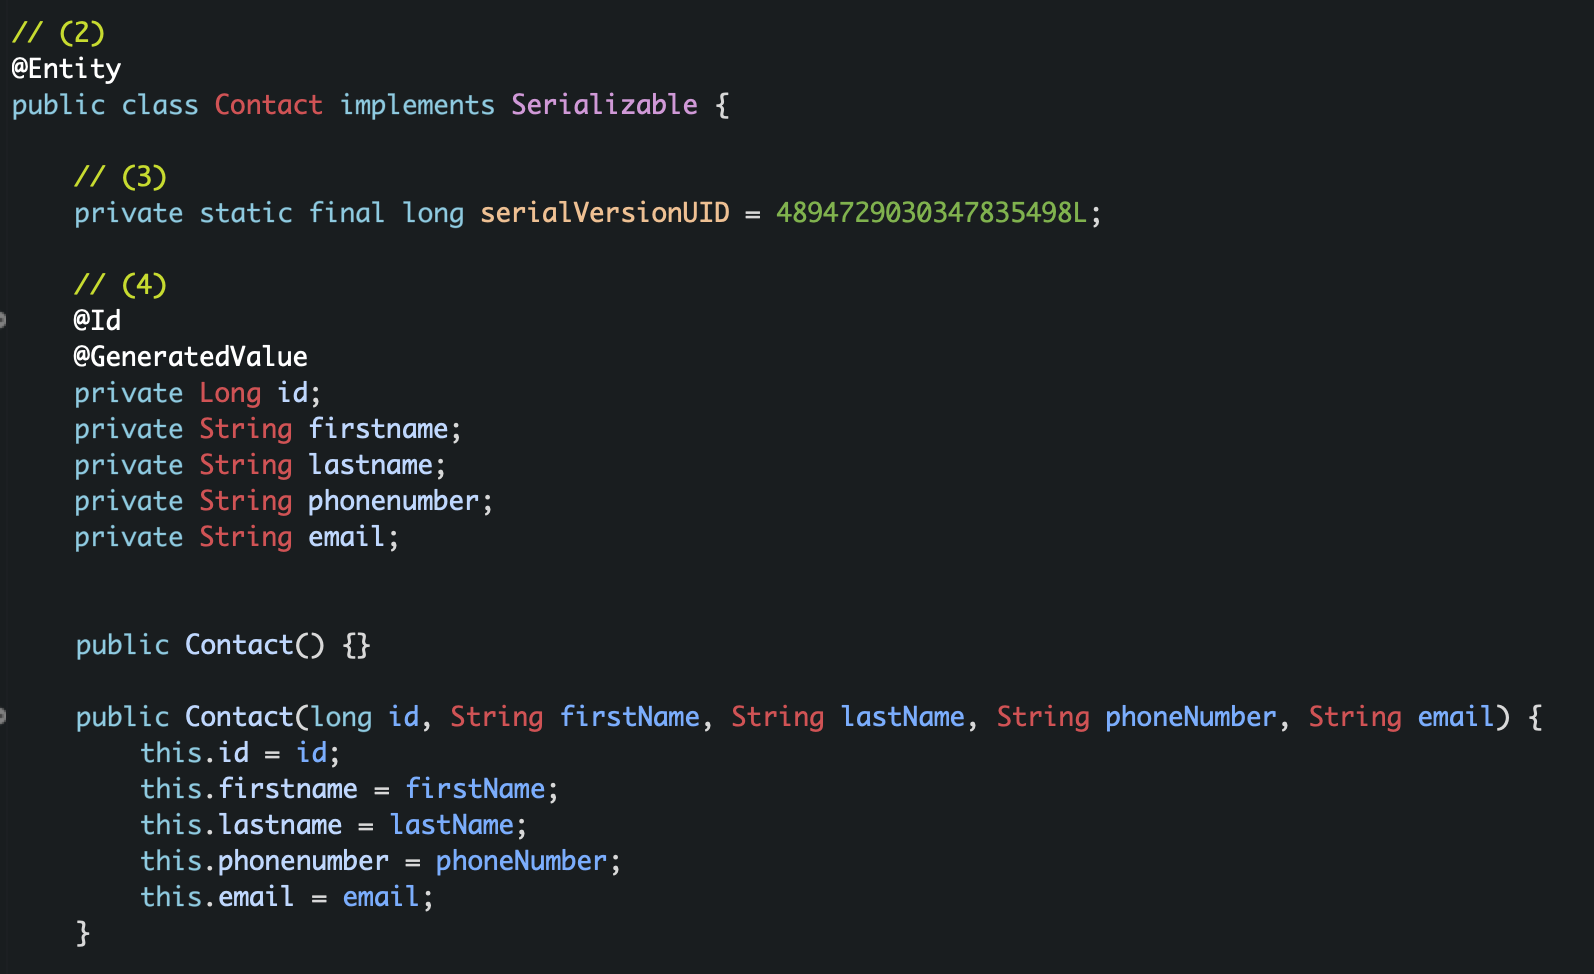
\includegraphics[width=6in]{figures/ContactsEntity.png}
        \caption{Entidad de Contactos}
    \end{figure}
\break
\break
    También se investigaron distintas formas de realizar el acceso a la base de datos desde el servidor pero finalmente nos decantamos por usar la
    clase \textbf{JPARepository} o \textbf{CRUDRepository}, las cuales nos ofrecen ya implementados los métodos típicos de las operaciones \textbf{CRUD}, además de la opción 
    de poder crear nuestros propios métodos.
\end{flushleft}

\begin{flushleft}
    Para poder probar las distintas peticiones de tipo \textbf{POST} y \textbf{GET}, que realizamos en local, usamos la herramienta 
    \textbf{Postman}, ver figura 3.7.
    \begin{figure}[H]
        \centering
        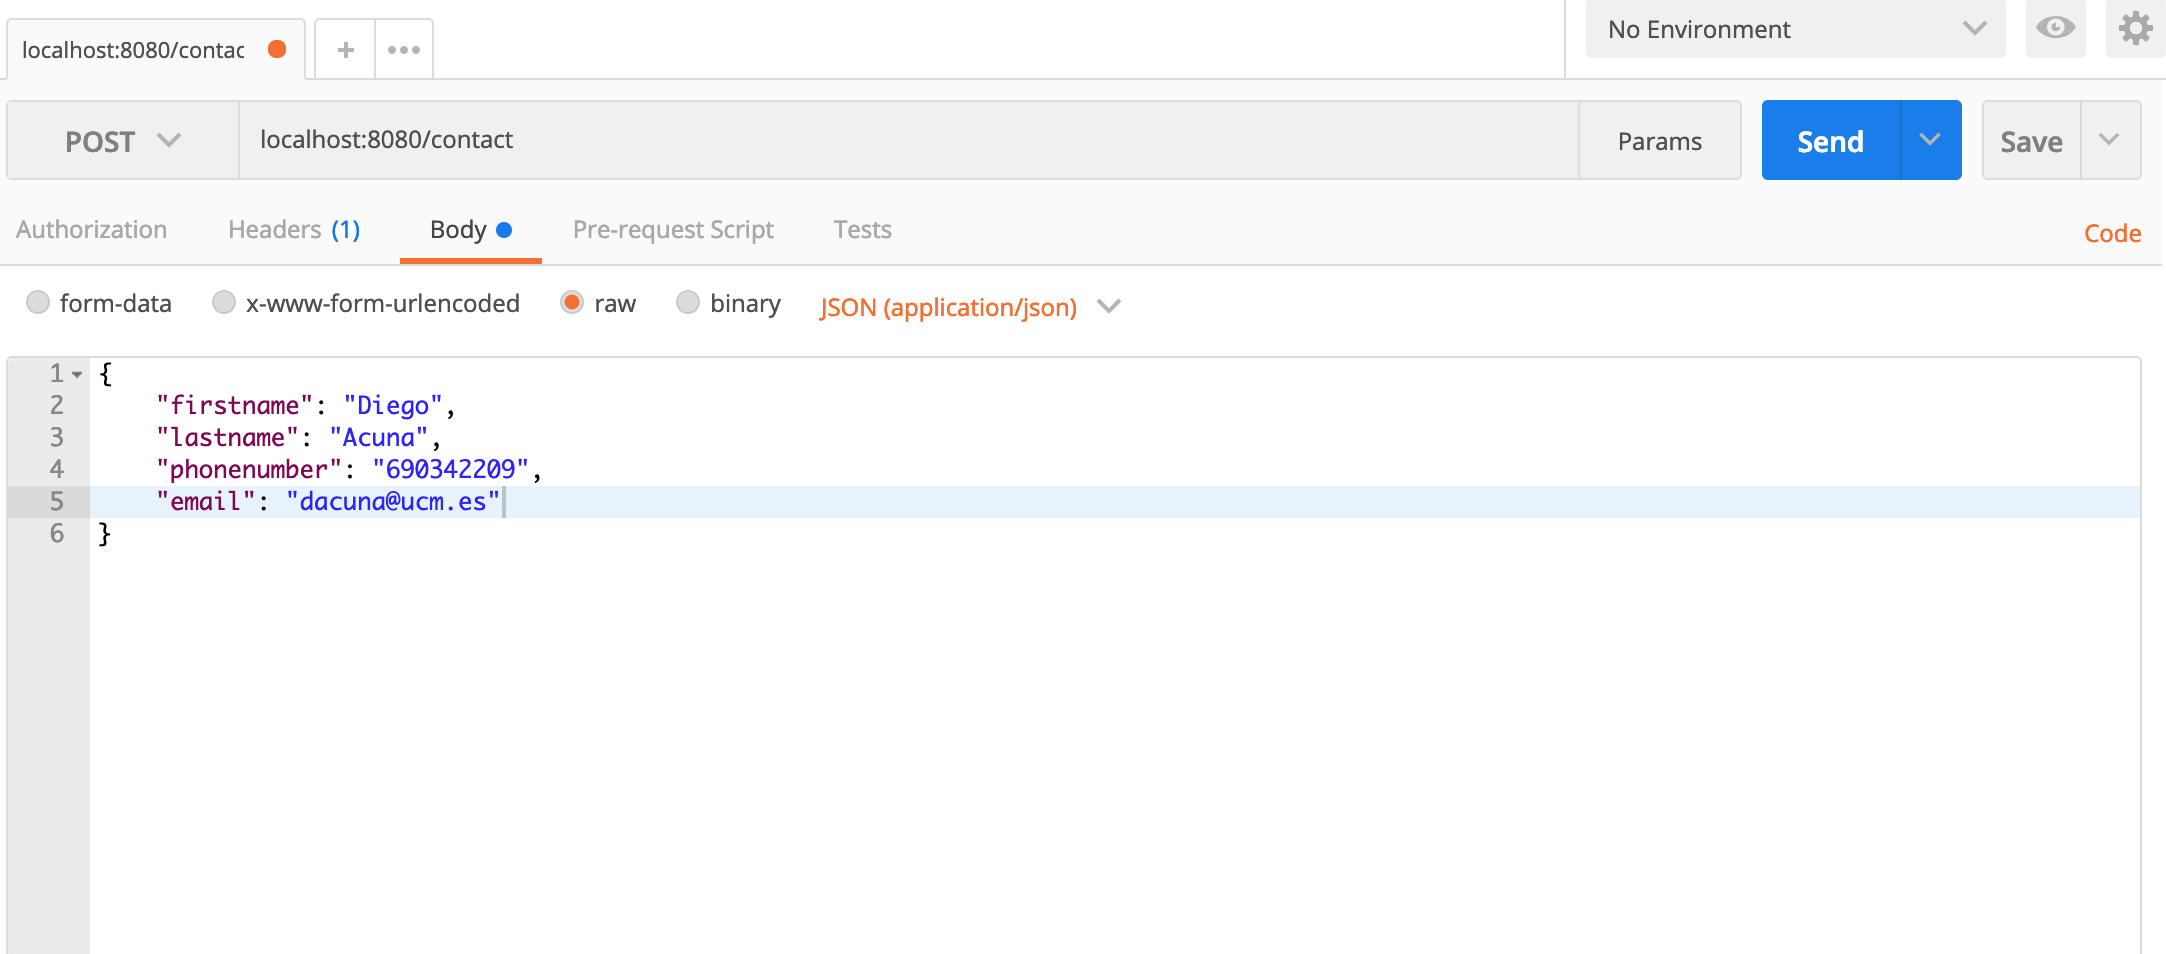
\includegraphics[width=6in]{figures/Postman.png}
        \caption{Postman}
    \end{figure}
    Para este prototipo decidimos usar \textbf{MySQL} como sistema de gestión de bases de datos relacional, aunque
    a la hora de probar a levantar nuestro servidor de prueba tuvimos que rehacer este prototipo, además de adaptarlo para 
    que gestionara entidades de películas, y que usara \textbf{PostgreSQL}, además de cambiar una serie de anotaciones y limpiar 
    el archivo \textbf{pom.xml} de líneas de código innecesarias, ver figura 3.8, que es el que contiene las dependencias de nuestro proyecto.
    \begin{figure}[H]
        \centering
        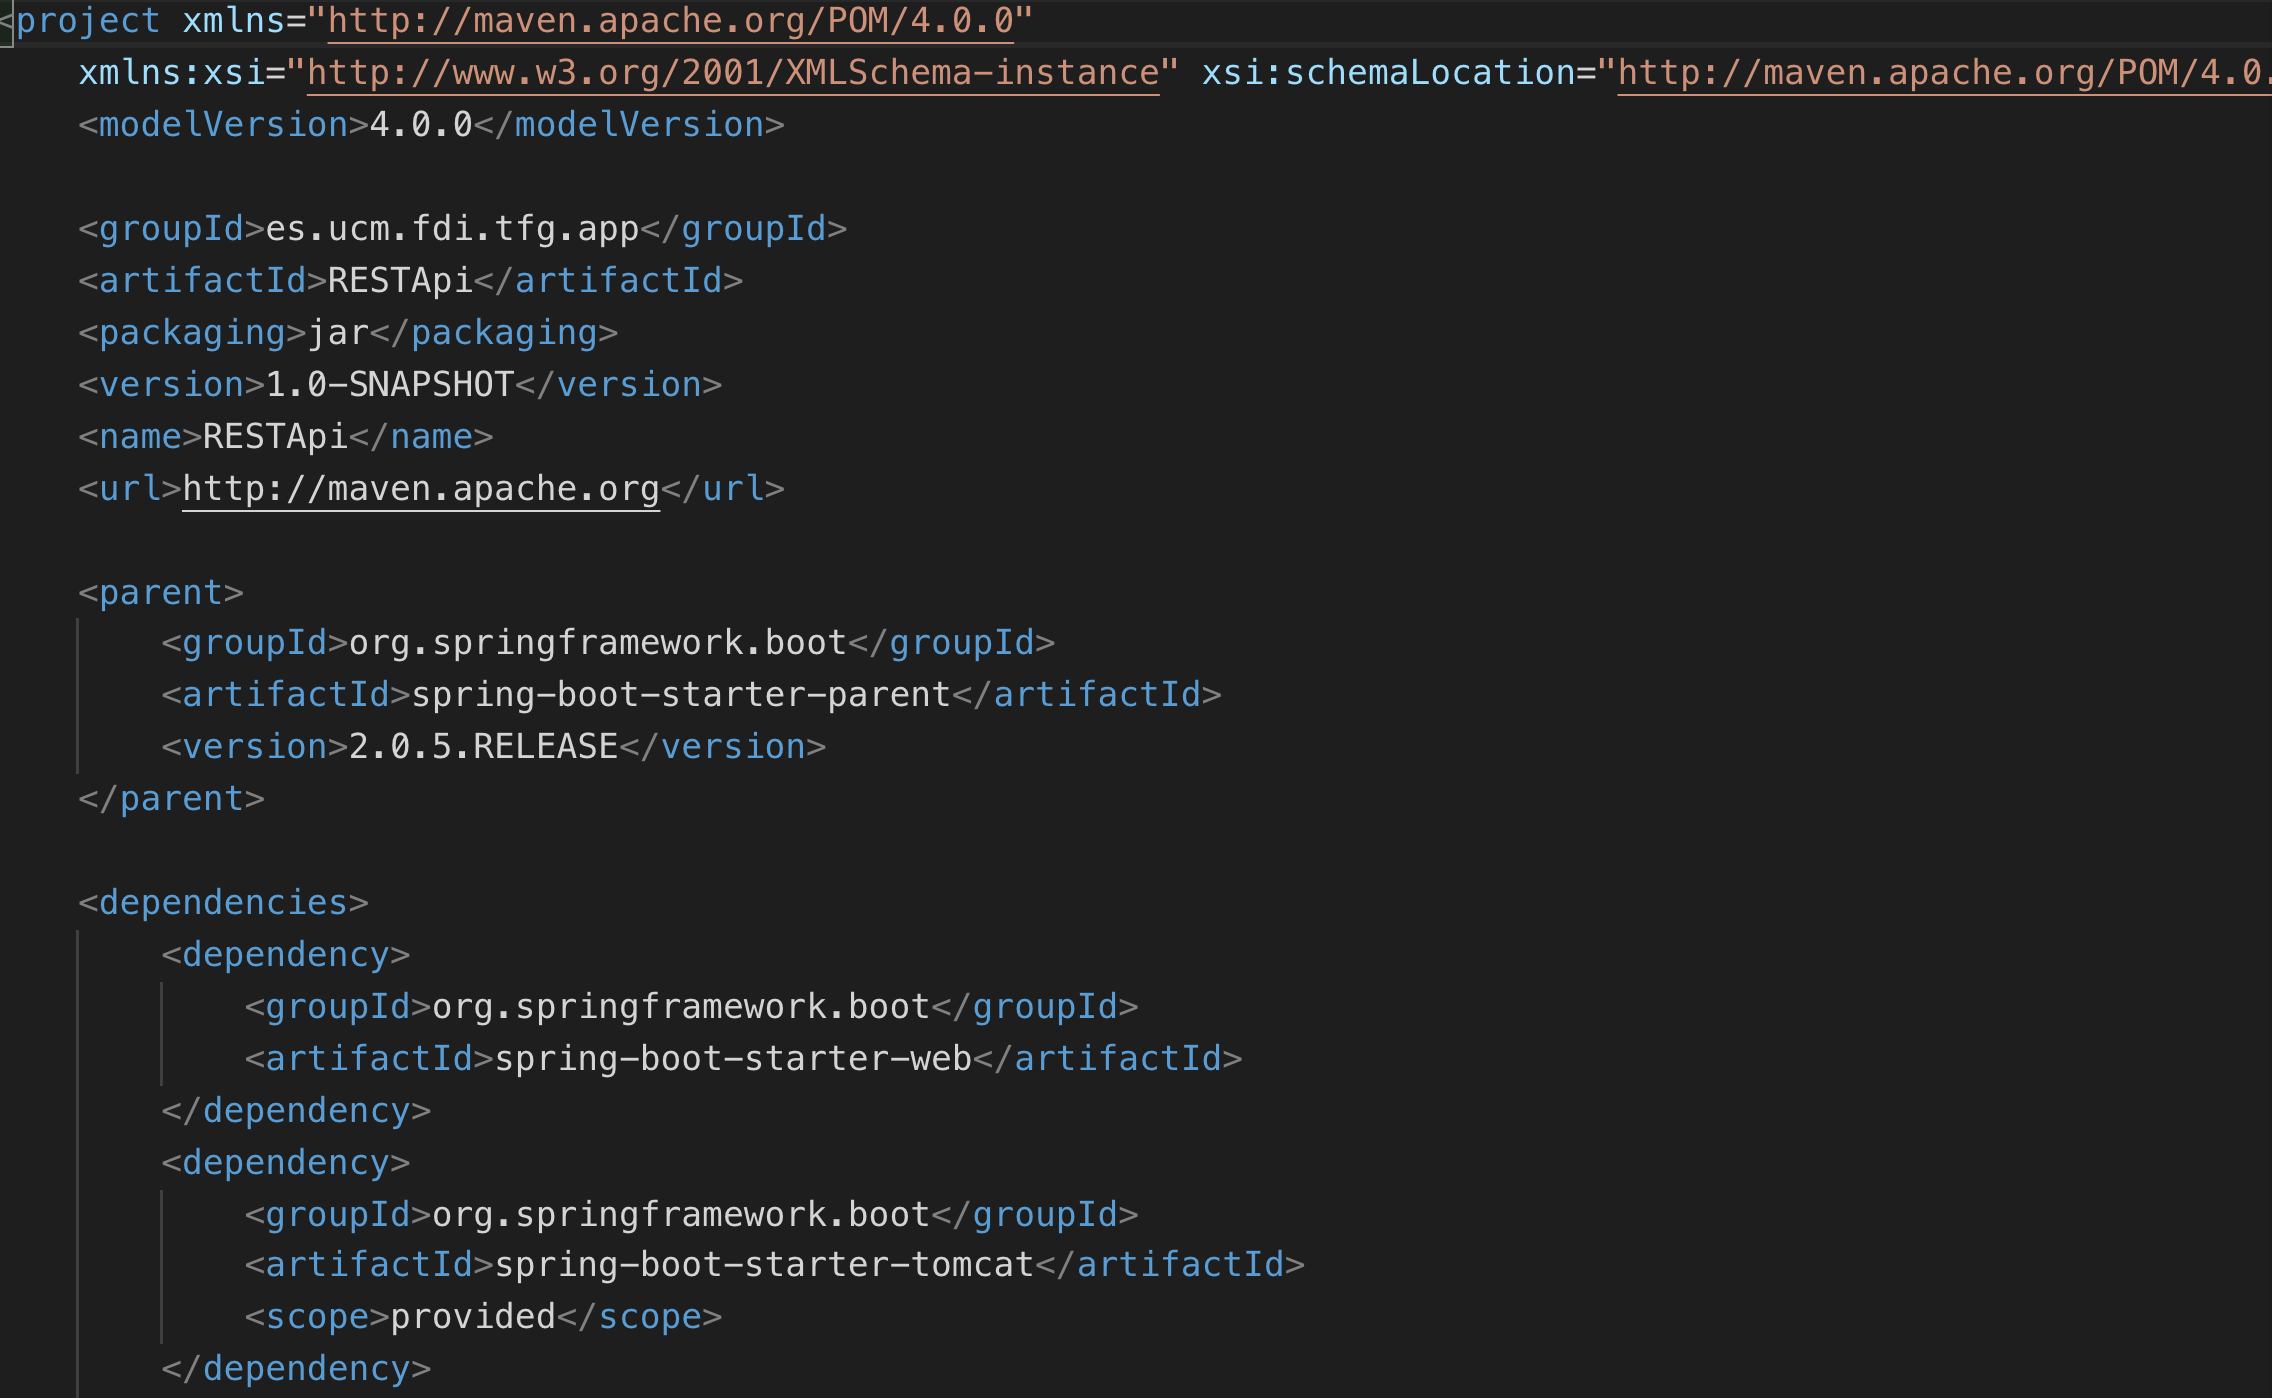
\includegraphics[width=6in]{figures/PomXML.png}
        \caption{Archivo pom.xml}
    \end{figure}
\end{flushleft}